\documentclass[T4paper.tex]{subfiles}

\begin{document}

%T4 Protein Figures
\begin{figure}[!ht]
\begin{subfigure}{\textwidth}
   \centering
   \frame{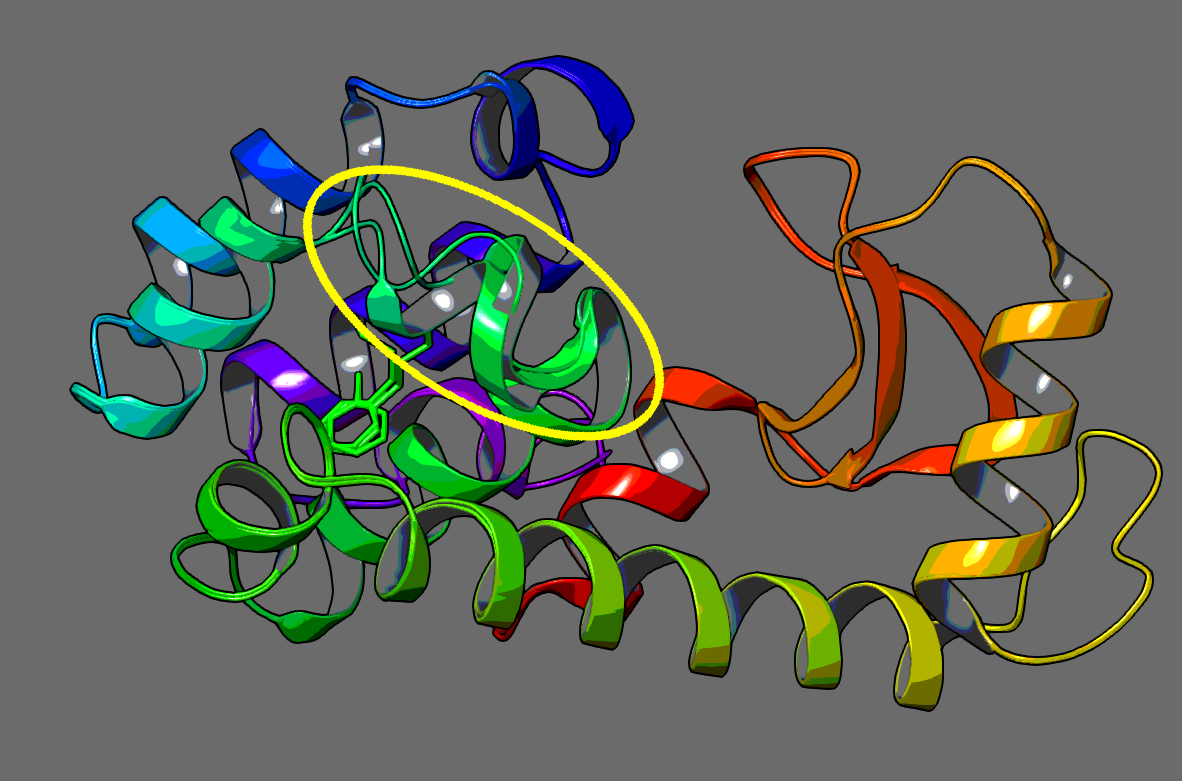
\includegraphics[width=\textwidth, height=0.3\textheight]{VMDscripts/Figures/T4_lysozyme_edit.png}}
   \caption{T4 lysozyme (L99A)}
   \label{fig:T4-L99A_protein}
\end{subfigure}
\centering
\begin{subfigure}{\textwidth}
  \centering
   \frame{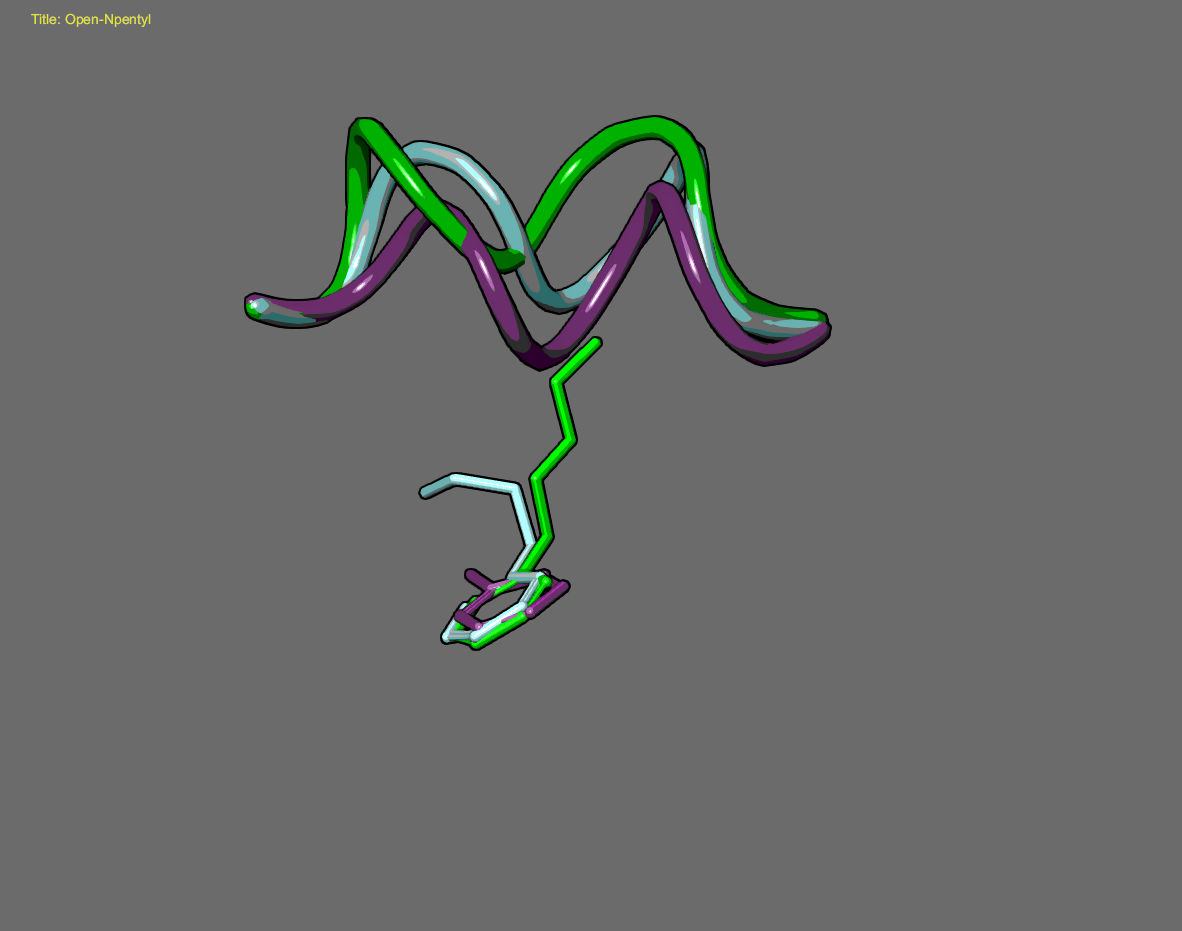
\includegraphics[trim={8cm 8cm 12cm 3cm}, clip, width=\textwidth, height=0.3\textheight]{VMDscripts/Figures/ProteinTube.png}}
   \caption{F-helix (residues 107-115)}
   \label{fig:T4-L99A_tube}
\end{subfigure}%
\caption{Fig.~\ref{fig:T4-L99A_protein} is a cartoon representation of the entire T4 lysozyme protein using protein-ligand bound crystal structures of the closed (PDB: 4W53), intermediate (PDB: 4W57), and open conformations (PDB: 4W59). Highlighted in yellow is the F-helix region spanning residues 107 to 115. In Fig.~\ref{fig:T4-L99A_tube} is closer view of strictly the F-helix in the closed (purple), intermediate (cyan), and open (green) conformational states and their corresponding ligands as found in their crystal structure positions. Images were created using Maestro\cite{Maestro}.}
\label{fig:T4-L99A}
\end{figure}
%%%%%%%%%%%%%%%%%%%%%%%%%%%%%%%%%%%%%%%

%Ligand occupancy/Exp Data
\begin{figure}[!ht]
   \frame{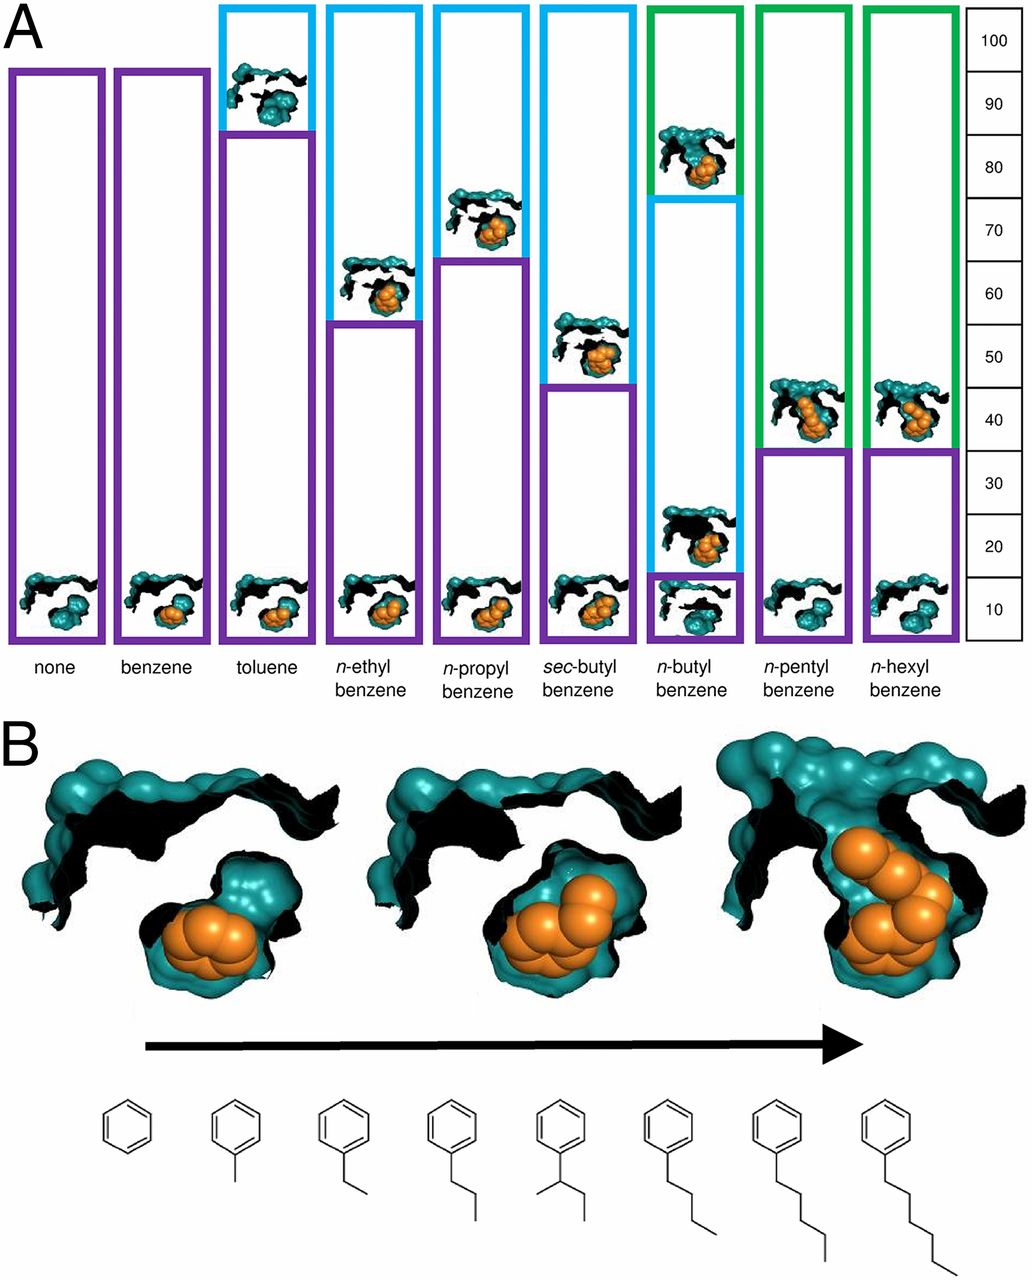
\includegraphics[width=\textwidth, height=0.75\textheight]{VMDscripts/Figures/F2large.jpg}}
   \caption{"Congeneric ligands are accommodated in L99A with conformational changes. (A) In the L99A cavity, the ligand poses were assigned to their respective protein conformations by matching the ligand occupancy with that of the F-helix conformation, which was typically unambiguous. (B) Molecular surface of the cavity, cut away to reveal the ligand (orange space-filling model), in examples of the closed (benzene complex), intermediate (ethylbenzene complex), and open (n-hexylbenzene complex) conformations. The full congeneric series is shown." Material adapted directly from a previous reported study conducted by Merski, et. al.\cite{Merski2015}. Information is summarized in Table~\ref{tbl:expdata}.}
   \label{fig:loop-occ}
\end{figure}
%%%%%%%%%%%%%%%%%%%%%%%%%%%%%%%%%%%%%%%%5

%F-helix and pREST residues
\begin{figure}[!h]
\begin{subfigure}{\textwidth}
   \centering
   \frame{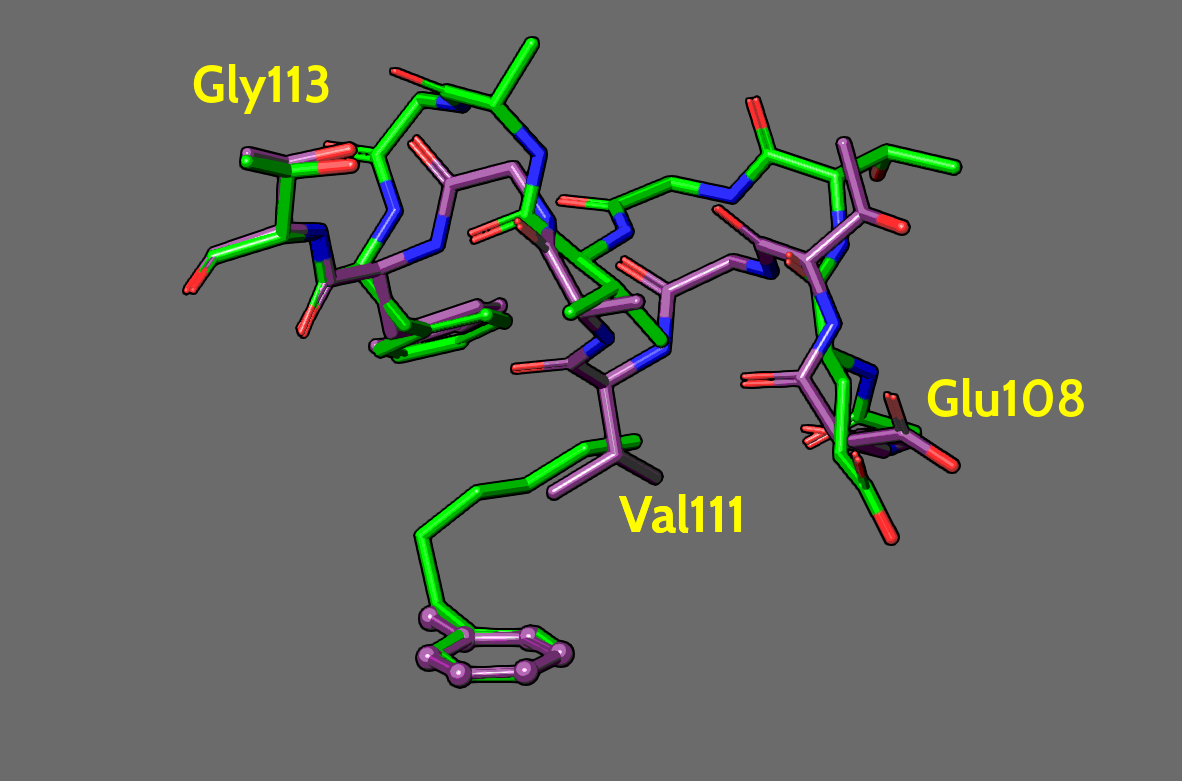
\includegraphics[trim={5cm 2cm 3cm 1cm}, clip, width=\textwidth, height=0.4\textheight]{VMDscripts/Figures/C2O.png}}
   \caption{Selected residues in pREST}
   \label{fig:C2O}
\end{subfigure}
\centering
\begin{subfigure}{.5\textwidth}
  \centering
   \frame{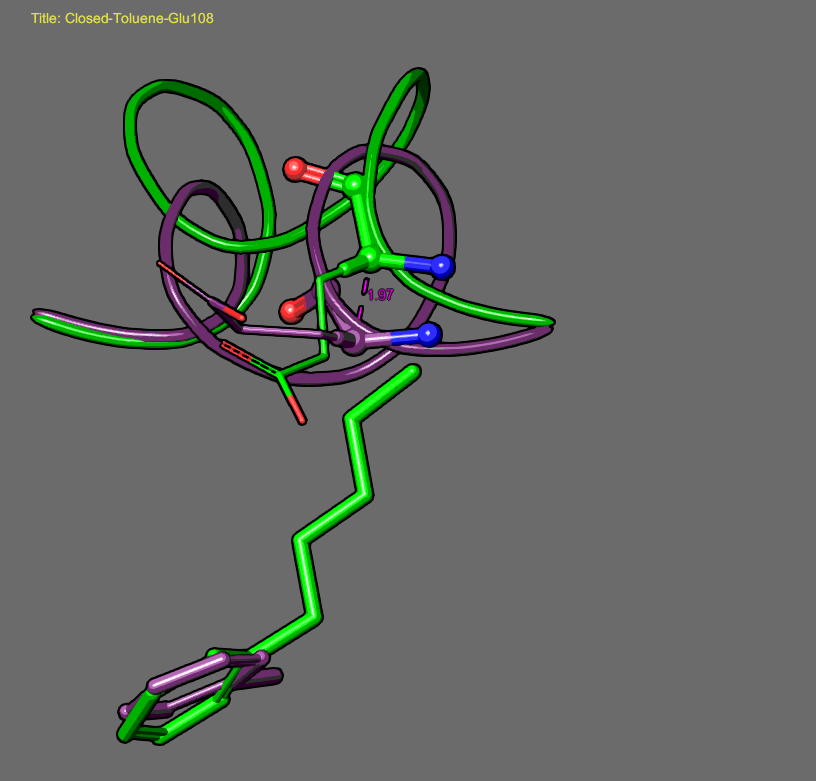
\includegraphics[trim={1cm 1cm 8cm 2cm}, clip, width=\textwidth, height=0.4\textheight]{VMDscripts/Figures/Glu108-C2O.png}}
   \caption{Residue Glu108}
   \label{fig:Glu108-C2O}
\end{subfigure}%
\begin{subfigure}{.5\textwidth}
   \centering
   \frame{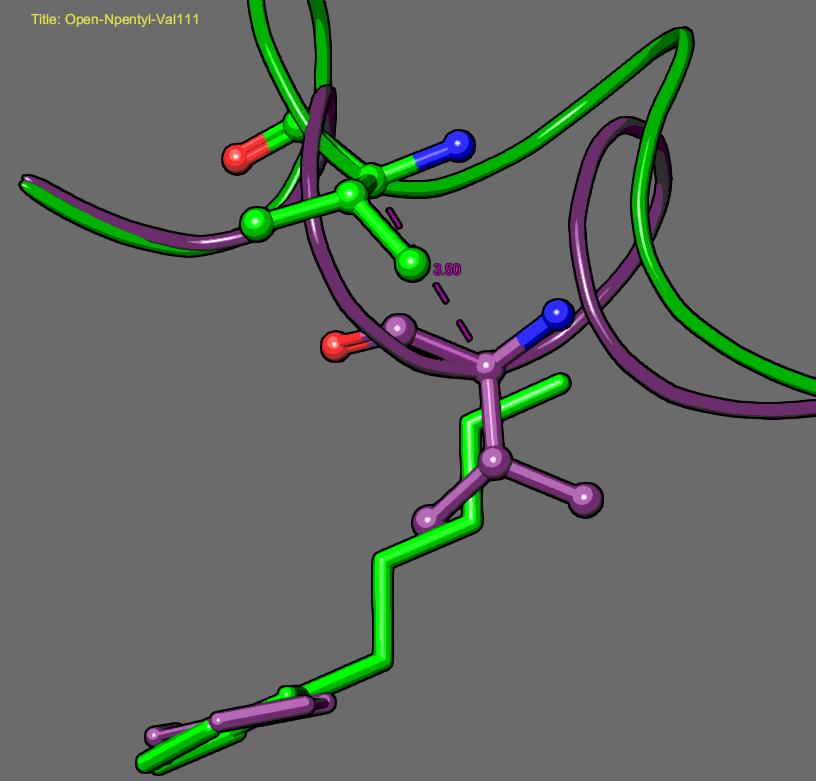
\includegraphics[trim={5cm 0cm 0cm 1cm}, clip, width=\textwidth, height=0.4\textheight]{VMDscripts/Figures/Val111-C2O.png}}
   \caption{Residue Val111}
   \label{fig:Val111-C2O}
\end{subfigure}
\caption{Fig.~\ref{fig:C2O} highlights the 3 residues selected to be included into the REST region for `pREST' simulations. Fig.~\ref{fig:Glu108-C2O} and Fig.~\ref{fig:Val111-C2O} illustrates the motion of the $C_{\alpha}$'s during the transition between the protein closed and open states, where the $C_{\alpha}$ in Glu108 undergoes a motion of approximately $2\AA$ and $3.5\AA$ in Val111.}
\label{fig:pRESTresidues}
\end{figure}
%%%%%%%%%%%%%%%%%%%%%%%%%%%%%%%%%%%%%%%%%%%%5

%RMSD/time plots
\begin{figure}[!h]
\begin{subfigure}{\textwidth}
   \centering
   \frame{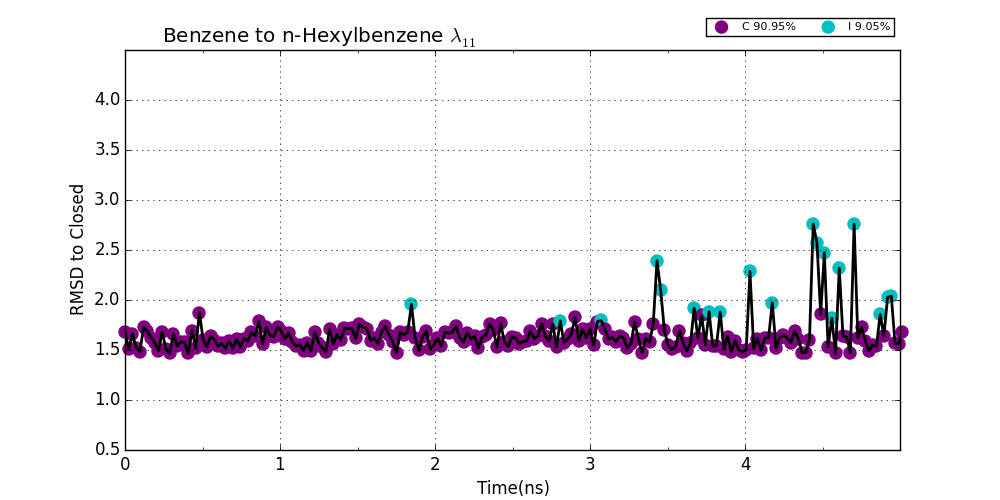
\includegraphics[trim={1.5cm 0 2cm 0.25cm}, clip, width=\textwidth, height=0.4\textheight]{VMDscripts/c_opls3_1/plots/0-5ns/RMSD-replica11.png}}
   \caption{Protein closed simulation}
   \label{fig:c_opls3_1/RMSD-replica11}
\end{subfigure}
\centering
\begin{subfigure}{\textwidth}
  \centering
   \frame{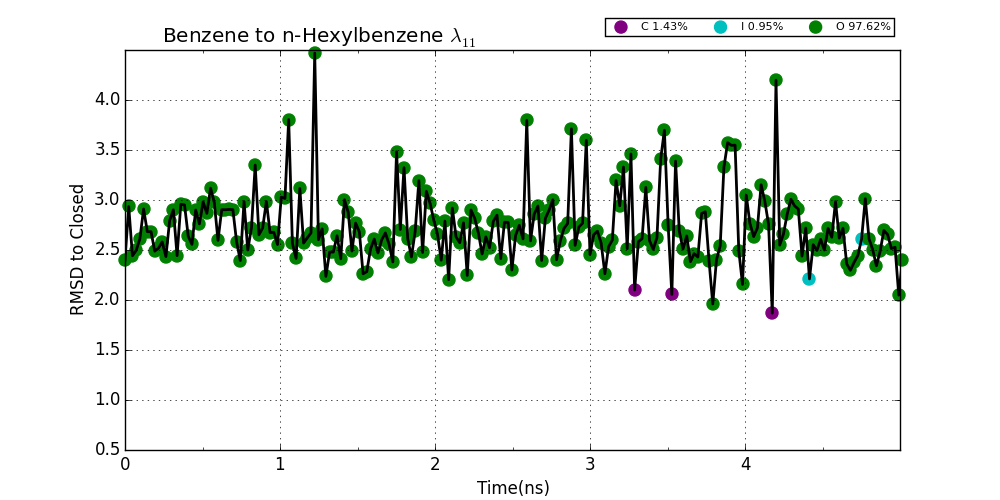
\includegraphics[trim={1.5cm 0 2cm 0.25cm}, clip, width=\textwidth, height=0.4\textheight]{VMDscripts/o_opls3_1/plots/0-5ns/RMSD-replica11.png}}
   \caption{Protein open simulation}
   \label{fig:o_opls3_1/RMSD-replica11}
\end{subfigure}%
\caption{Plotted is the RMSD relative to the closed helix conformation (black line), where each time point is colored according to the protein state of lowest RMSD to the trajectory. Here, using the default protocol in the transformation of benzene to n-hexylbenzene, RMSD/time plots correspond to the final end state of n-hexylbenzene ($\lambda_{11}$). Fig.~\ref{fig:c_opls3_1/RMSD-replica11} corresponds to the simulation that began from the protein closed state and Fig.~\ref{fig:o_opls3_1/RMSD-replica11} is from the simulation started from the protein open state. The legends indicate the percentage of sampling of each protein conformational state from the trajectory.}
\label{fig:benzene_to_n-hexyl}
\end{figure}

\begin{figure}[!h]
\begin{subfigure}{\textwidth}
   \centering
   \frame{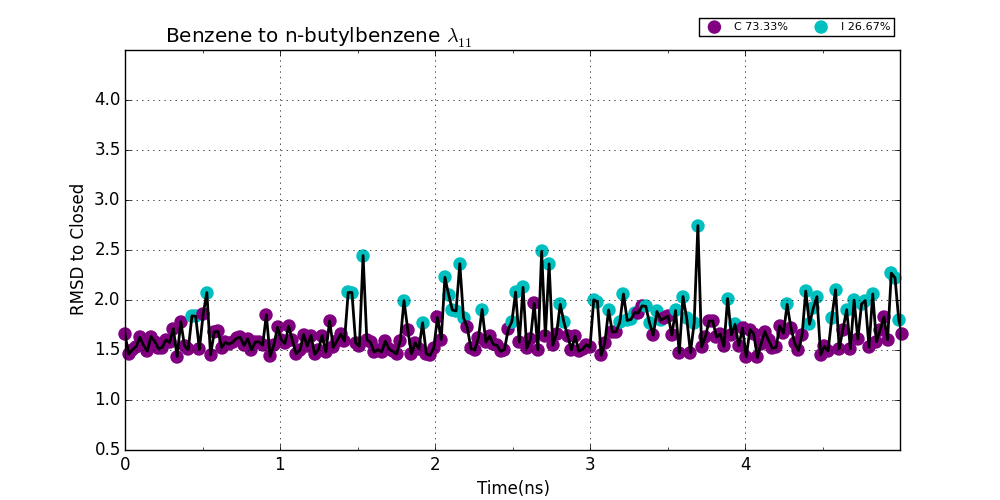
\includegraphics[trim={1.5cm 0 2cm 0.25cm}, clip, width=\textwidth, height=0.4\textheight]{VMDscripts/c_exp_opls3_11/plots/0-5ns/RMSD-replica11.png}}
   \caption{Protein closed simulation}
   \label{fig:c_exp_opls3_11/RMSD-replica11}
\end{subfigure}
\centering
\begin{subfigure}{\textwidth}
  \centering
   \frame{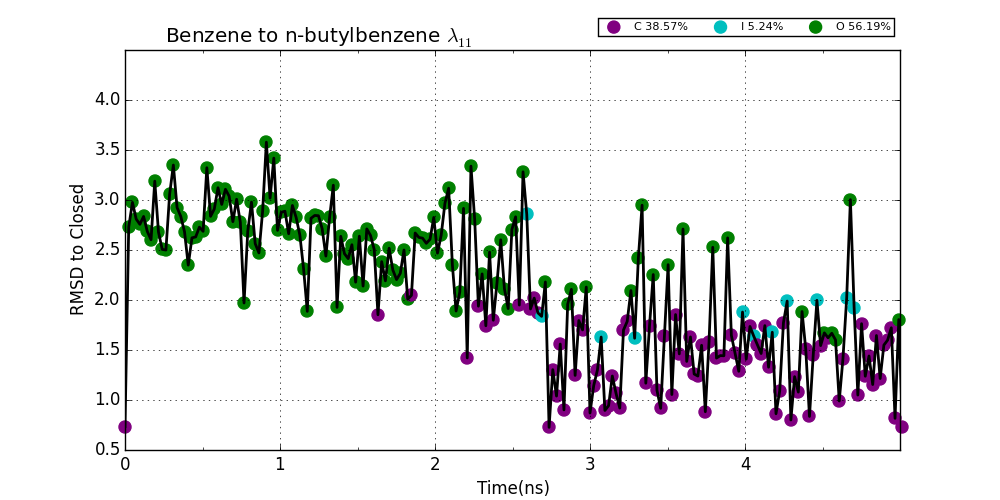
\includegraphics[trim={1.5cm 0 2cm 0.25cm}, clip, width=\textwidth, height=0.4\textheight]{VMDscripts/o_exp_opls3_24/plots/0-5ns/RMSD-replica11.png}}
   \caption{Protein open simulation}
   \label{fig:o_exp_opls3_24/RMSD-replica11}
\end{subfigure}%
\caption{RMSD/time plots correspond to the final end state of n-butylbenzene ($\lambda_{11}$) while using the default protocol for transformation of benzene to n-butylbenzene. Fig.~\ref{fig:c_exp_opls3_11/RMSD-replica11} and Fig.~\ref{fig:o_exp_opls3_24/RMSD-replica11} 
correspond to simulations that were started from the protein closed or open state, respectively. The legends indicate the percentage of sampling of each protein conformational state from the trajectory.}
\label{fig:benzene_to_n-butyl}
\end{figure}

\begin{figure}[!h]
\begin{subfigure}{\textwidth}
   \centering
   \frame{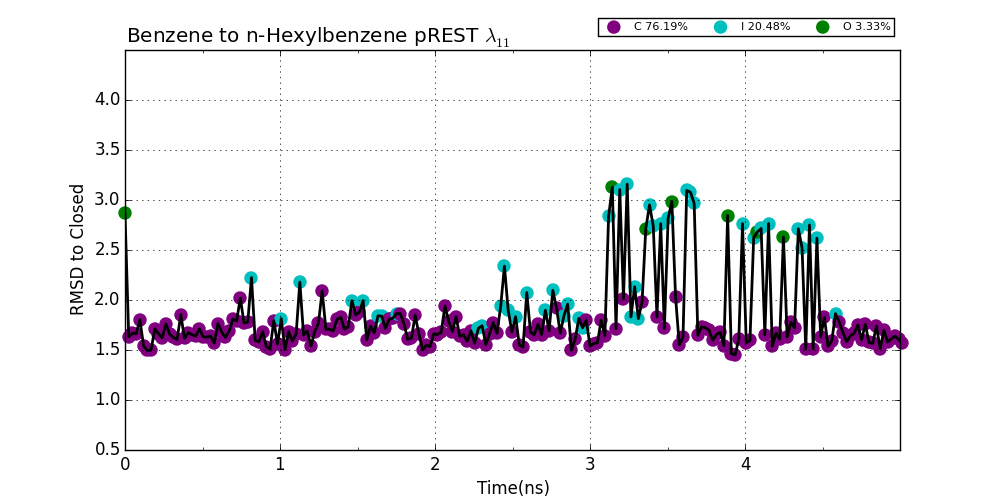
\includegraphics[trim={1.5cm 0 2cm 0.25cm}, clip, width=\textwidth, height=0.4\textheight]{VMDscripts/c_opls3_rest1_extend_1e/plots/0-5ns/RMSD-replica11.png}}
   \caption{Protein closed simulation, pREST}
   \label{fig:c_opls3_rest1_1/RMSD-replica11}
\end{subfigure}
\centering
\begin{subfigure}{\textwidth}
  \centering
   \frame{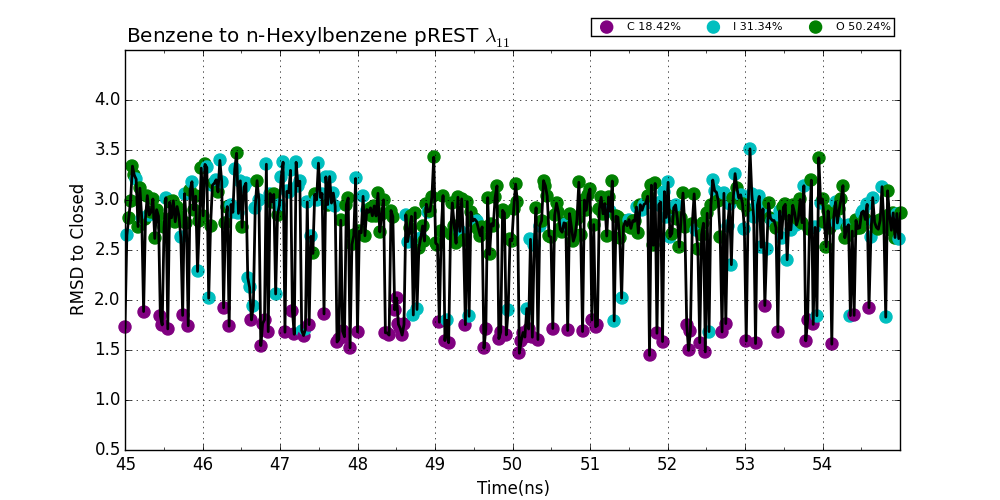
\includegraphics[trim={1.5cm 0 2cm 0.25cm}, clip, width=\textwidth, height=0.4\textheight]{VMDscripts/c_opls3_rest1_extend_1e/plots/45-55ns/RMSD-replica11.png}}
   \caption{Protein closed simulation, pREST extended}
   \label{fig:c_opls3_rest1_1/45-55ns/RMSD-replica11}
\end{subfigure}%
\caption{Using the modified REST region (pREST) in the transformation of benzene to n-hexylbenzene, we plot the RMSD/time corresponding to the n-hexylbenzene state ($\lambda_{11}$) with the simulation starting from protein closed for the first 5ns (Fig.~\ref{fig:c_opls3_rest1_1/RMSD-replica11}) and the final 10ns from an extended run up to 55ns (Fig.~\ref{fig:c_opls3_rest1_1/45-55ns/RMSD-replica11}).}
\label{fig:benzene_to_n-hexyl_pREST}
\end{figure}
%%%%%%%%%%%%%%%%%%%%%%%%%%%%%%%%%%%%%%%%%%%%%%%%%%%%%%

%COLOR MAPS
\begin{figure}[!h]
\begin{subfigure}{.5\textwidth}
  \centering
   \frame{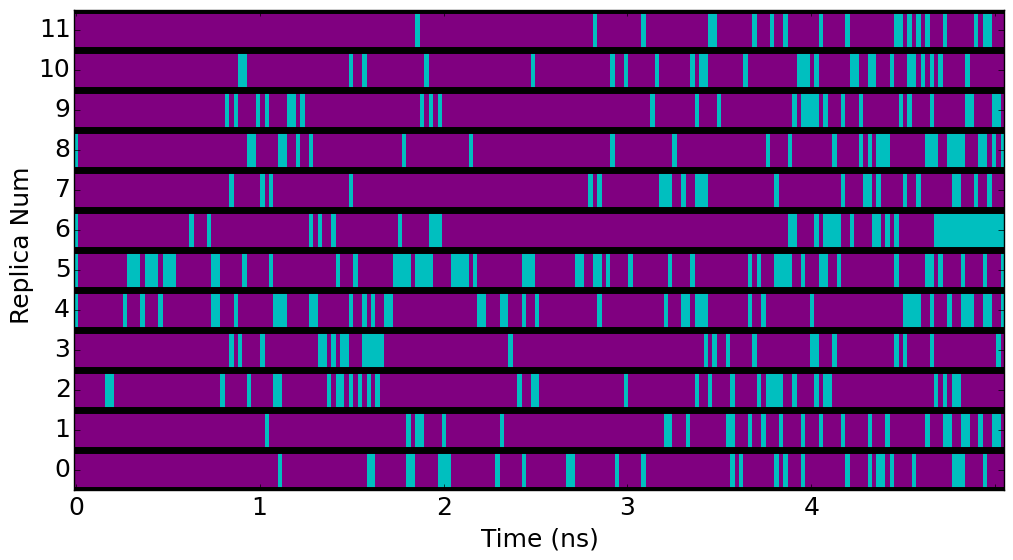
\includegraphics[width=\textwidth, height=0.4\textheight]{VMDscripts/c_opls3_1/plots/colormap/cmap-0-5ns.png}}
   \caption{Default}
   \label{fig:c_opls3_1/colormap}
\end{subfigure}%
\begin{subfigure}{.5\textwidth}
   \centering
   \frame{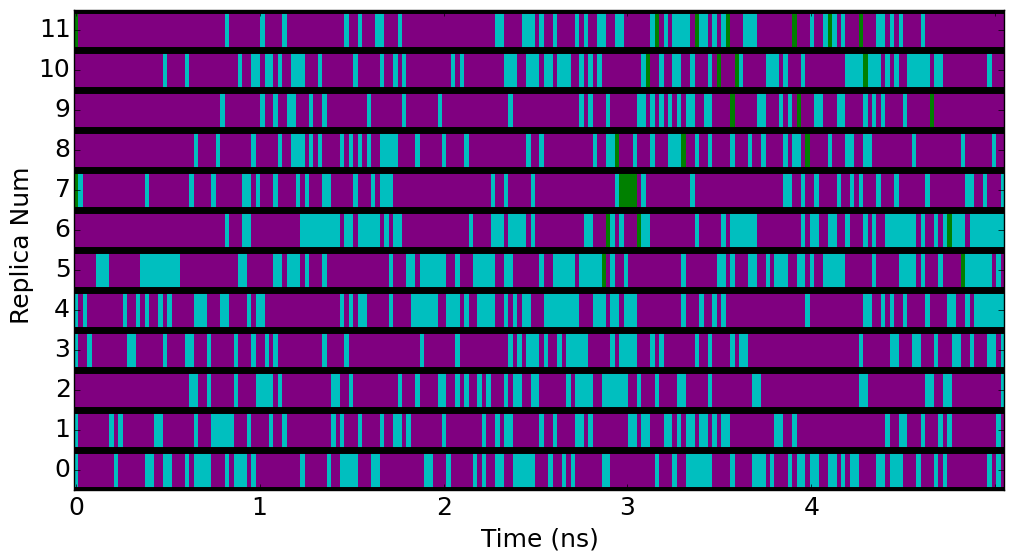
\includegraphics[width=\textwidth, height=0.4\textheight]{VMDscripts/c_opls3_rest1_extend_1e/plots/colormap/cmap-0-5ns.png}}
   \caption{pREST}
   \label{fig:c_opls3_rest1_1/colormap}
\end{subfigure}
\centering
\begin{subfigure}{\textwidth}
   \centering
   \frame{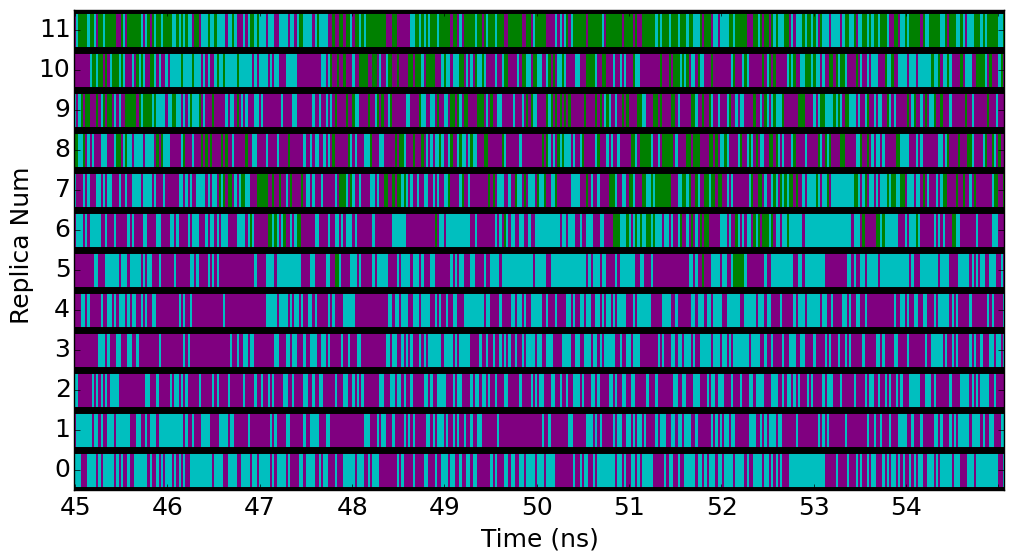
\includegraphics[clip, width=\textwidth, height=0.4\textheight]{VMDscripts/c_opls3_rest1_extend_1e/plots/colormap/cmap-45-55ns.png}}
   \caption{pREST extended}
   \label{fig:c_opls3_rest1_1/cmap-45-55ns}
\end{subfigure}
\caption{Color maps of simulations starting from the protein closed state for the benzene to n-hexylbenzene alchemical transformation. Lines at every frame are colored accordingly to the protein state of lowest RMSD (purple-closed, cyan-intermediate, green-open). Fig.~\ref{fig:c_opls3_1/colormap} corresponds to simulations using the default protocol. Fig.~\ref{fig:c_opls3_rest1_1/colormap} represents simulations using the modified REST region protocol (pREST). Fig.~\ref{fig:c_opls3_rest1_1/cmap-45-55ns} illustrates the enhancement in protein conformational sampling through extending the pREST simulation time up to 55ns. }
\label{fig:benzene_to_n-hexyl_colormap}
\end{figure}
%%%%%%%%%%%%%%%%%%%%%%%%%%%%%%%%%%%%%%%%%%%%%%

%XYPlots
\begin{figure}[!h]
\centering
\begin{subfigure}{.5\textwidth}
  \centering
   \frame{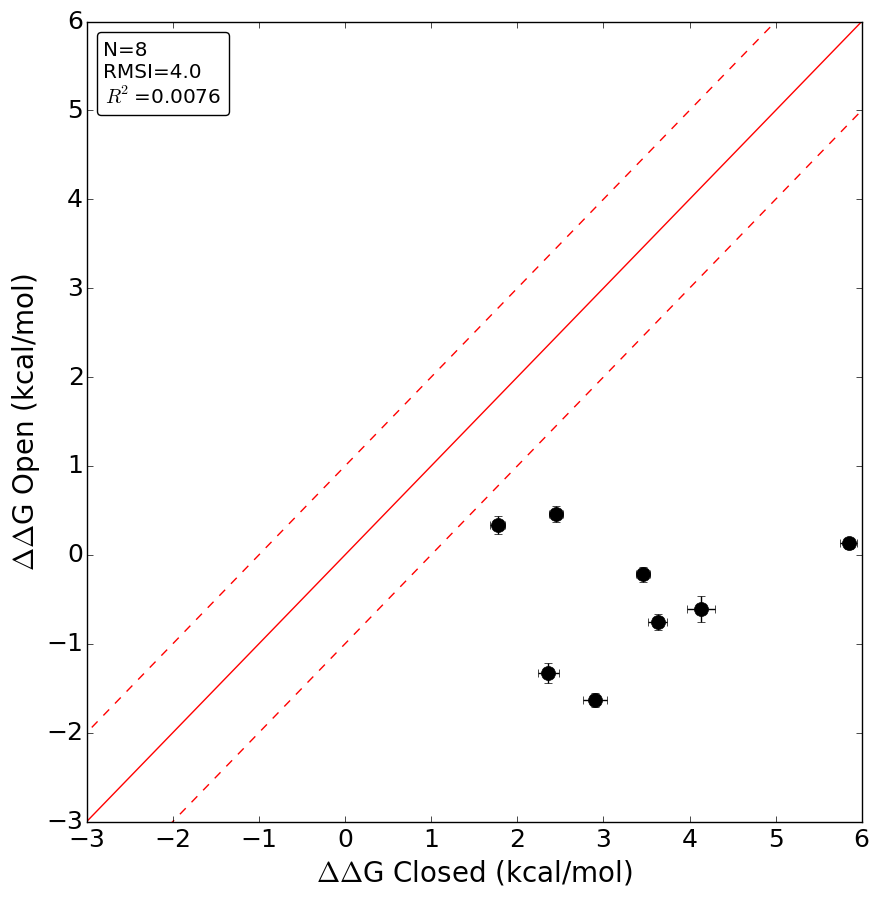
\includegraphics[width=\textwidth, height=0.3\textheight]{VMDscripts/XYplot/C2O_xyplot.png}}
   \caption{Closed-Open: Default}
   \label{fig:C2O_xyplot}
\end{subfigure}%
\begin{subfigure}{.5\textwidth}
   \centering
   \frame{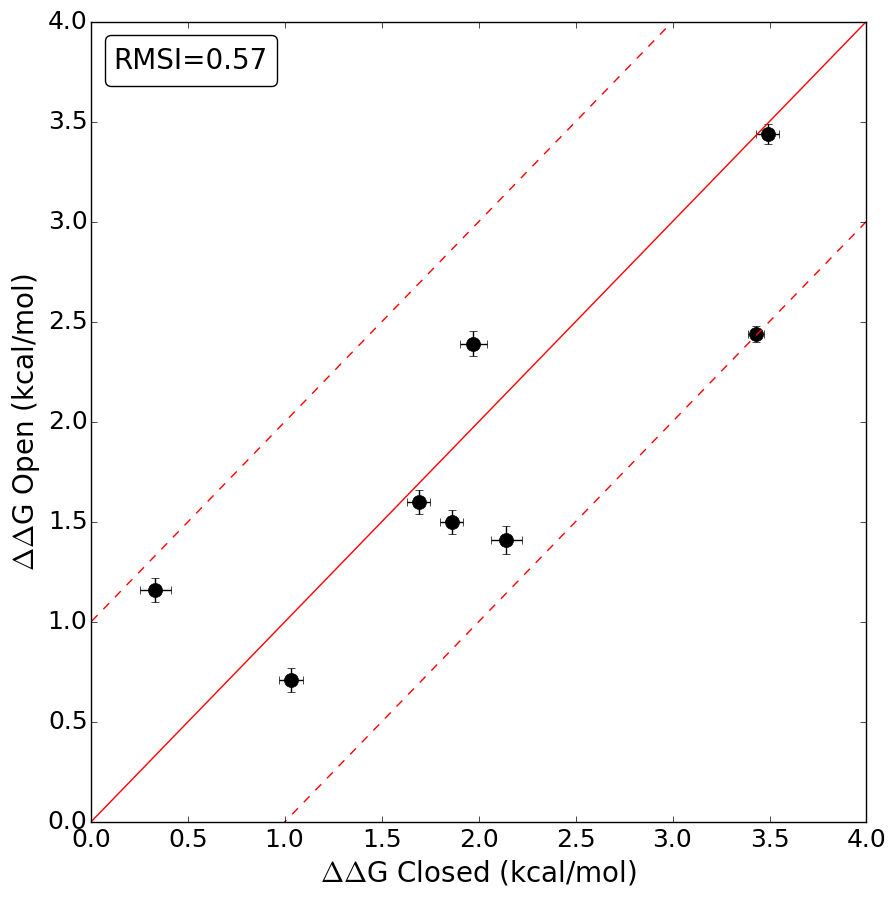
\includegraphics[width=\textwidth, height=0.3\textheight]{VMDscripts/XYplot/C2O_pREST_xyplot.png}}
   \caption{Closed-Open: pREST}
   \label{fig:C2O_xyplot_pREST}
\end{subfigure}
\centering
\begin{subfigure}{.5\textwidth}
  \centering
   \frame{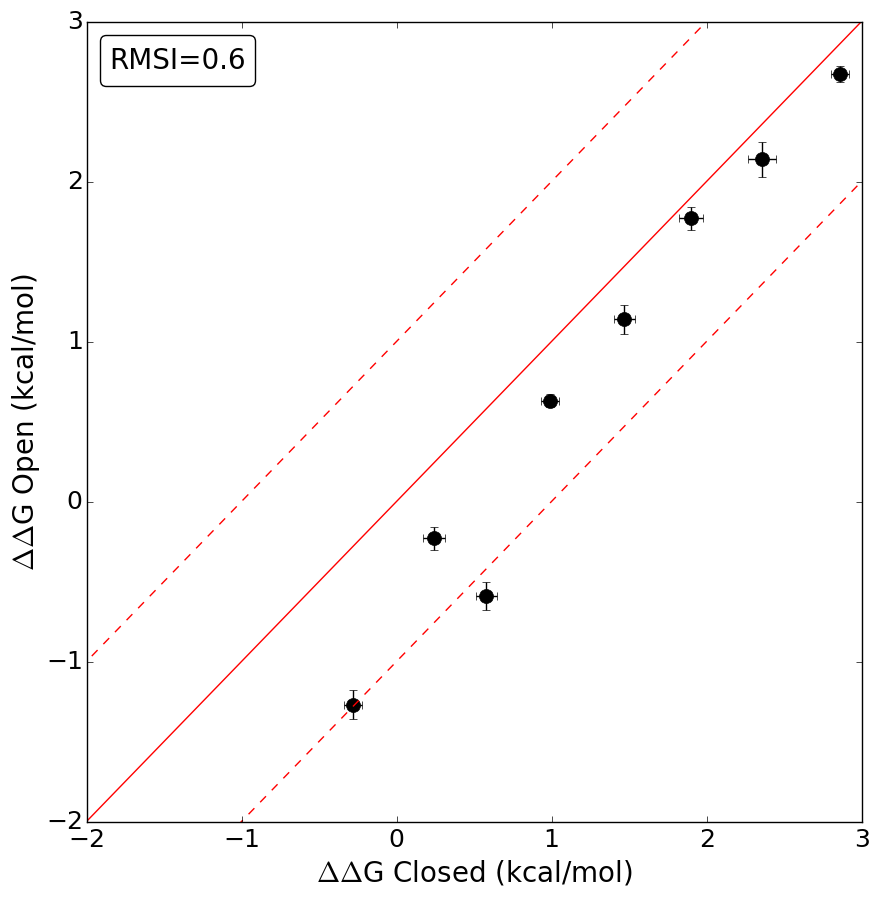
\includegraphics[width=\textwidth, height=0.3\textheight]{VMDscripts/XYplot/C2I_xyplot.png}}
   \caption{Closed-Intermediate: Default}
   \label{fig:C2I_xyplot}
\end{subfigure}%
\begin{subfigure}{.5\textwidth}
   \centering
   \frame{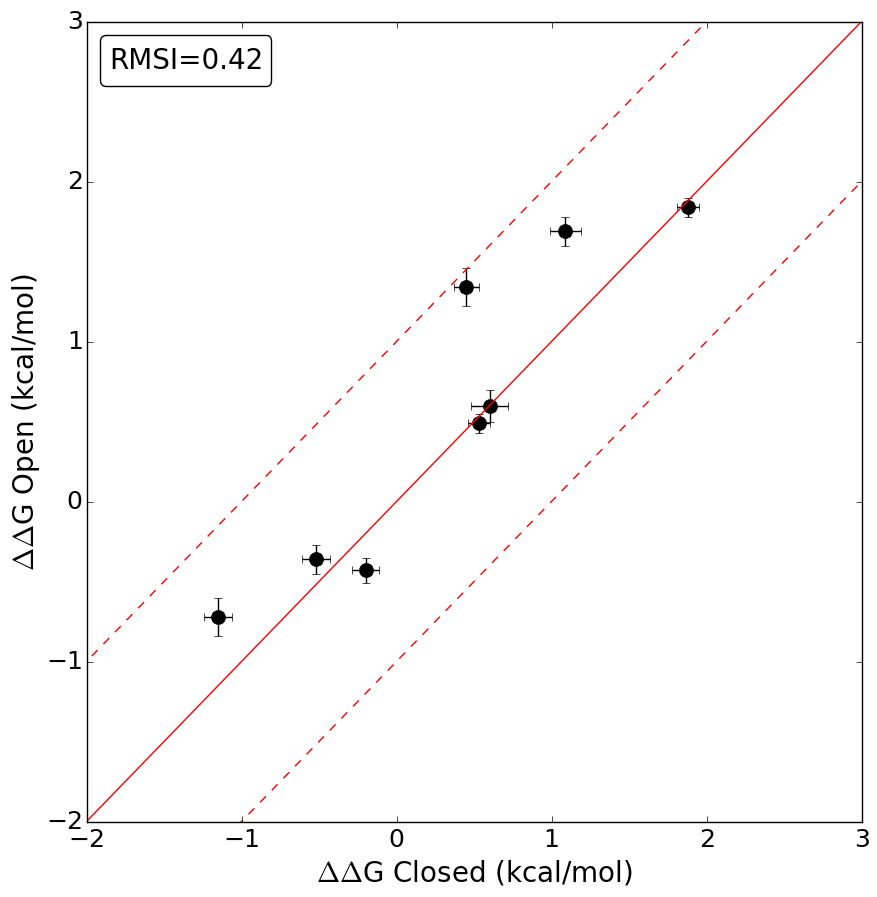
\includegraphics[width=\textwidth, height=0.3\textheight]{VMDscripts/XYplot/C2I_pREST_xyplot.png}}
   \caption{Closed-Intermediate: pREST}
   \label{fig:C2I_xyplot_pREST}
\end{subfigure}
\caption{$\Delta\Delta G_{calc}$ from MD simulations beginning from the protein closed versus open state. Fig.~\ref{fig:C2O_xyplot} plots relative free energies obtained using the default protocol from the `closed-open' alchemical transformations set, yielding a RMSI of 4.0 kcal/mol and in Fig.~\ref{fig:C2O_xyplot_pREST} are the final computed free energies with simulations carried out to 55ns using pREST, giving RMSI of 0.57 kcal/mol. Similarly, Fig.~\ref{fig:C2I_xyplot} plots relative free energies from the `closed-intermediate' set using the default protocol which gives an RMSI of 0.6 kcal/mol and in Fig.~\ref{fig:C2I_xyplot_pREST} are  free energies with simulations carried out up to 25ns using pREST, giving RMSI of 0.42 kcal/mol. Tables containing the numerical data for each plot can be found in the supplementary information.}
\label{fig:conf-xyplots}
\end{figure}

\begin{figure}[!h]
\centering
\begin{subfigure}{.5\textwidth}
  \centering
   \frame{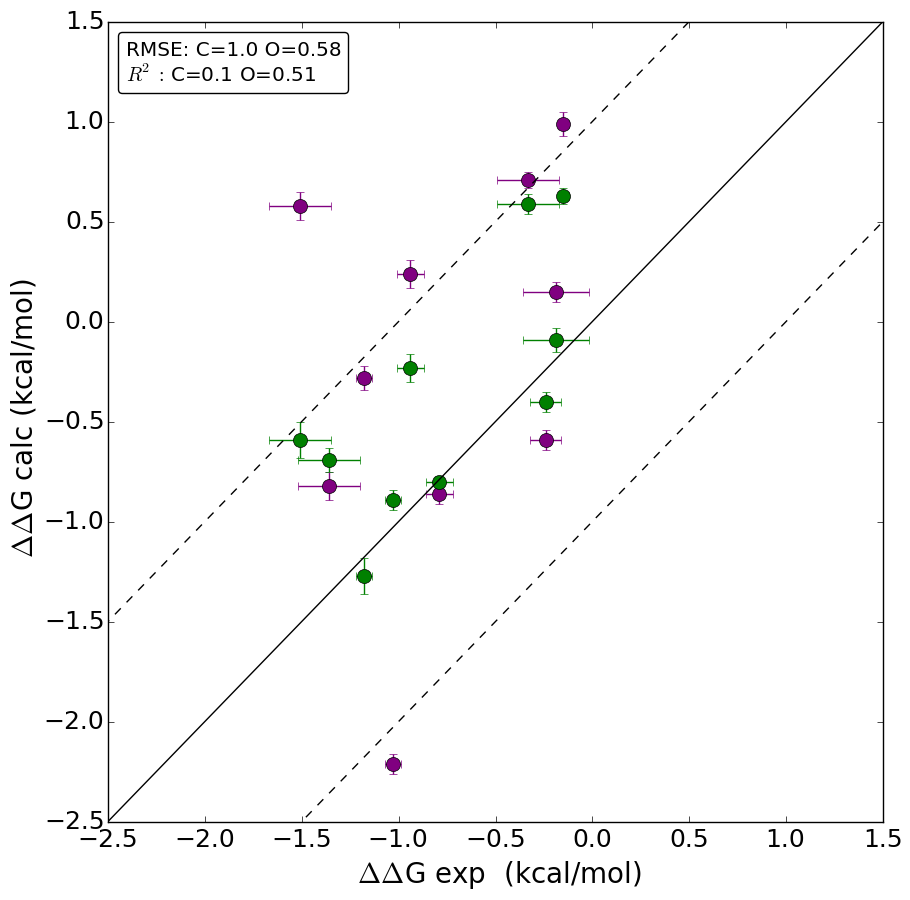
\includegraphics[width=\textwidth, height=0.3\textheight]{VMDscripts/XYplot/exp_xyplot.png}}
   \caption{Default}
   \label{fig:exp_xyplot}
\end{subfigure}%
\begin{subfigure}{.5\textwidth}
   \centering
   \frame{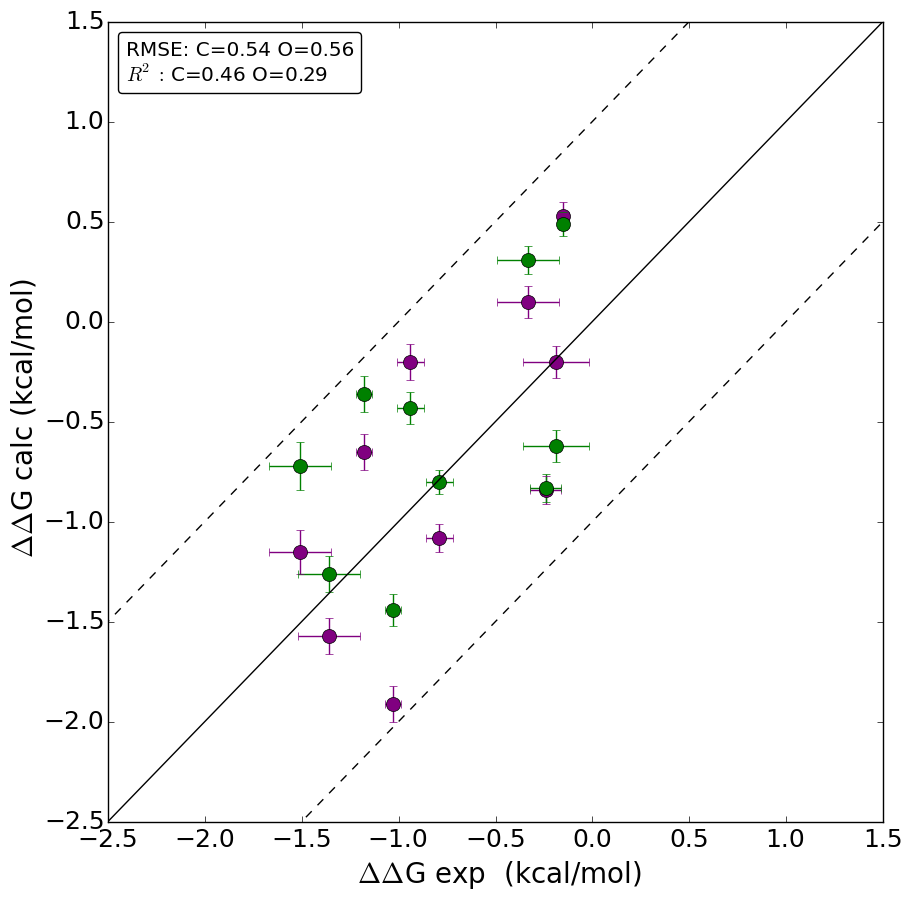
\includegraphics[width=\textwidth, height=0.3\textheight]{VMDscripts/XYplot/exp_pREST_xyplot.png}}
   \caption{pREST}
   \label{fig:exp_xyplot_pREST}
\end{subfigure}
\caption{$\Delta\Delta G_{calc}$ from MD simulations beginning from the protein closed (purple) and open (green) state compared against $\Delta\Delta G_{exp}$. Fig.~\ref{fig:exp_xyplot} plots free energies obtained using the default protocol which gives a 1.0 kcal/mol and 0.58 kcal/mol RMSE for protein closed and open simulations, respectively. Fig.~\ref{fig:exp_xyplot_pREST} plots the final free energies after applying pREST, yielding an RMSE of 0.54 for protein closed and 0.56 kcal/mol for protein closed simulations.} 
\label{fig:exp-xyplots}
\end{figure}
%%%%%%%%%%%%%%%%%%%%%%%%%%%%%%%%%%%%%%%%%%%%%%%%


\end{document}